%\documentclass{sig-alternate}

%%%%%%%%%%%%%%%%%%%%%%%%%%%%%%%%
% comment out the following to switch back to sig-alternate!!
\documentclass[11pt]{article}
\usepackage[margin=1in]{geometry}
\usepackage{booktabs,tabularx}
\usepackage{fullpage}
\usepackage{times}
\usepackage{url}
\usepackage{epsfig}
%\usepackage{subfigure}
\usepackage{makecell}
\usepackage{graphicx}
\usepackage{titlesec}
\usepackage{multirow}
\usepackage{amsmath, amsthm, amssymb}

\titlespacing{\section}{0pt}{3mm}{1mm}
\titlespacing{\subsection}{0pt}{2mm}{0.5mm}
\titlespacing{\subsubsection}{0pt}{2mm}{0.8mm}
% done with the part that should be commented out!
%%%%%%%%%%%%%%%%%%%%%%%%%%%%%%


\usepackage{algorithm}
\usepackage{algorithmic}
\usepackage{listings}
\usepackage{times}
\usepackage{graphicx}
\usepackage{listings}
\usepackage{courier}
\usepackage{times}
\usepackage[T1]{fontenc}
\usepackage{cleveref}
\usepackage{amsmath}
\usepackage{caption}
\usepackage{amssymb}
\usepackage{latexsym}
\usepackage{bm}
\usepackage{color}
\usepackage{subscript}
\usepackage{multirow}
\usepackage{multicol}
\usepackage{tgheros}
\usepackage{array}
\usepackage{verbatim}

\newcounter{Examplecount}
\setcounter{Examplecount}{0}
\newenvironment{example}
{\stepcounter{Examplecount} {\bf Example} \arabic{Examplecount} \begin{it}}{\end{it} }

%\newcommand{\muhat}{\hat{\mu}}
%\newcommand{\sigmahat}{\hat{\sigma}}
%\newcommand{\todo}[1]{[\textbf{TODO: #1}]}
%\newcommand{\eat}[1]{} % TO MAKE LARGE BLOCKS OF TEXT INVISIBLE
%\newcommand{\sz}[1]{\lvert#1\rvert}
%\newcommand{\card}[1]{\lvert#1\rvert}
%\newcommand{\xp}[2]{P \if*#1\else^{#1}\fi \if*#2\else_{\! #2}\fi}
%\newcommand{\pr}[3]{\xp{#1}{#2}\left\{\,#3\,\right\}}
%\newcommand{\prl}[3]{\xp{#1}{#2}\{\,#3\,\}}
%\renewcommand\:{\colon} % for use with \sset, etc.
%\newcommand{\sset}[1]{\left\{\,#1\,\right\}}
%\newcommand\xD{\mathcal{D}}
%\newcommand\xP{\mathcal{P}}
%\newcommand\xS{\mathcal{S}}
%\newcommand\xbar{\bar x}
%\newcommand\vbar{\bar v}
%\newcommand\xmax{{x_{\text{max}}}}
%\newcommand\eps{\epsilon}
%\newcommand{\eeblk}{\hbox{\lower 1pt \vbox{\hrule width6pt\hbox to
%  6pt{\vrule height5pt depth1pt \hfil\vrule height5pt depth1pt} \hrule
%  width6pt} \unskip}}
%\newcommand{\eblk}{{\unskip\nobreak\hfil\penalty50
%  \hskip1em\hbox{}\nobreak\hfil\eeblk
%  \parfillskip=0pt\finalhyphendemerits=0\par}}
%\newtheorem{xample}{Example}
\makeatletter
\newenvironment{sql}%
 {\vspace{-3 pt} \begin{list}{}{%
  \setlength{\topsep}{0pt}\setlength{\partopsep}{0pt}\setlength{\parskip}{0pt}%
  \setlength{\parsep}{0pt}\setlength{\labelwidth}{0pt}%
  \setlength{\rightmargin}{0pt}\setlength{\leftmargin}{0pt}%
  \setlength{\labelsep}{0pt}%
  \obeylines\@vobeyspaces\normalfont\ttfamily%
  \item[]}}
 {\end{list}\vspace{-3 pt}\noindent}
\makeatother
%\newcommand{\bpar}[1]{\vskip 5pt\noindent\textbf{#1}\hskip 1em}
%\newcommand\yN{{\tilde N}}
%\newcommand\yX{{\tilde X}}
%\newcommand\ymu{{\tilde\mu}}
%\newcommand\ysigma{{\tilde\sigma}}

%\newcommand{\goodgap}{
%        \hspace{\subfigtopskip}
%        \hspace{\subfigbottomskip}
%}

%\newtheorem{definition}{Definition}
%\newtheorem{Rule}{Rule}
%\newtheorem{lemma}{Lemma}
%\newtheorem{theorem}{Theorem}
%\newtheorem{problem}{Problem}
%\newtheorem{example}{Example}
%\newtheorem{optimization}{Optimization}
%\newtheorem{observation}{Observation}
%\newtheorem{corollary}{Corollary}

\hyphenation{par-am-et-rize par-am-et-riz-ed}

\begin{document}
\clubpenalty=10000 
\widowpenalty = 10000


\begin{center}{\textbf{Data Management Plan}}\end{center}

$$P(\theta | \Psi) = \prod_i \textrm{Normal}(f_{t(\theta_i)}(\theta_i) | \Psi, \sigma_{t(\theta_i)})$$

$$f$$

$$P(\Psi | \theta)$$ 

$$P(F | \Psi)$$

The proposed project will develop software implementing PLinyCompute, as described in
this proposal. The software and testbeds will be developed, managed, distributed, and supported as a collaborative software
project, with a view towards an open source release when the research has been completed. Components of the system
will be distributed under GPL, BSD and EPL licenses, depending on the provenance of any external open source
code used. All code will be preserved and maintained for a minimum of three years beyond the award period
as required by NSF guidelines. Based on our experience with past projects, we expect the code to be preserved for
a much longer duration.
All electronic data will be preserved in multiple on-site backups in the form of DVDs and RAID hard drive
storage. Copies of the electronic data will be preserved off-site at Rice University's storage facilities. If requested,
access to the data will be provided via contact with the PI. Data will be available for access and sharing as soon as
is reasonably possible, and no later than two years after its acquisition. The data will be preserved for at least three
years beyond the award period, as required by NSF guidelines.
We do not anticipate that there will be any significant intellectual property issues involved with the acquisition of
the data. In the event that discoveries or inventions are made in direct connection with this data, access to the data
will be granted upon request once appropriate invention disclosures and/or provisional patent filings are made.
The data acquired and preserved in the context of this proposal will be further governed by Rice University's
policies pertaining to intellectual property, record retention, and data management.



\clearpage
\setcounter{page}{1}

\begin{center}
\textbf{Postdoctoral Mentoring Plan}
\end{center}

The presence of a postdoctoral researcher is essential in this project
because of its broad scope. This person will ideally have previous
training in systems and/or database research, 
and will be
able to grasp from the very beginning the broader goals of the project
and help the Ph.D. students who will be recruited for this
project. 
He or she will work closely with PI Jermaine.
This person will also gain an
understanding of issues related to the collaborations with graduate students.
and dissemination of software as discussed under the Broader Impacts.
Specifics of the training program include the following:

\vspace{-5pt}\paragraph{Orientation}
Discuss the postdoc's expectations of the mentor/mentee relationship, the source of funding for the postdoc's compensation, and the scientific and educational goals of the 
project.  
\vspace{-5pt}\paragraph{Building trust}
Ask the postdoc about his/her goals and respect and accept them where
these are reasonable; if not reasonable, attempt to steer the postdoc to
more realistic goals.  
Encourage feedback from the postdoc regarding his/her need for guidance.
Watch for depression, fatigue, isolation.

\vspace{-5pt}\paragraph{Education/training}
Explicitly instruct the postdoc in research methodology and techniques,
effective problem-solving strategies, and critical interpretation of the 
scientific literature.  Inform the postdoc of available resources and be 
willing to refer him/her to someone else for help/information.
Discuss a timeline for progress in the research project.
Encourage the postdoc to seek additional mentors in the various areas
in which s/he will require guidance.
Involve the postdoc in establishing successful collaborations.
Promote ethical standards for conducting research including compliance
with all institutional and federal regulations as they relate to responsible
conduct in research.
% Define expectations for the ethical conduct of
% research.
% Discuss the ground rules of collaboration; clarify collaborative
% issues such as ownership and sharing of research results and proper
% attribution of contributions to the research.  
% Discuss conflict of interest, grant applications, and ethical
% implications of the postdoc's research.
% Involve the postdoc in scientific discussions within group meetings
% and/or on an individual basis.
Provide opportunities for the postdoc to participate in the writing
and reviewing of papers and grant applications.  
% Encourage the postdoc to take the time to attend meetings, seminars
% and other career development activities, maintaining an appropriate balance
% between these activities and the development of the postdoc's research 
% career.
% Establish and communicate rules of authorship.
% Ensure that the research performed by a postdoc is submitted for
% publication in a timely manner and that s/he receives appropriate credit for
% the work performed.  
% Encourage creativity and independence.
\vspace{-3pt}
\paragraph{Evaluation}
Conduct periodic reviews with the postdoc.
% Assess the postdoc's progress to date, strengths, areas needing
% improvement, and potential for a research career in the discipline.
Maintain open communication with the postdoc regarding career goals
and options. %Include a periodic review of mutual expectations.
Offer candid assessment of the postdoc's potential to become
an independent investigator.
\vspace{-3pt}

\paragraph{Career preparation}
%Support/encourage the postdoc to present their work at scientific
%meetings. 
Help the postdoc engage in networking; introduce him/her to
colleagues at meetings or by phone/email.
Play an active role in the postdoc's job search (provide advice on
applications, CVs, interviews, presentations, negotiations, etc.).
Offer opportunities for the postdoc to develop supervisory skills
through training students and other research staff.
% Encourage the postdoc to participate in career development seminars
% and activities offered by Rice University.
Encourage the postdoc to actively seek opportunities for professional
experience and advancement (e.g., volunteer on committees, organize
scientific meetings/retreats).
% Maintain a positive attitude toward a diverse range of career
% opportunities for the postdoc; learn about nonacademic opportunities and
% provide appropriate advice for postdocs interested in nontraditional career
% paths.
In addition to the mentoring provided within the proposed project,  
Rice University offers exceptional opportunities for the training of the
postdoctoral researcher. These include:
\begin{itemize}
\item Participation in NSF ADVANCE activities which include lunches on issues that concern postdoctoral students and an annual very successful workshop ``Negotiating the Ideal Faculty Position.''
\item Rice's Grant writing workshop for NSF.
\item Rice's training in using large clusters and facilities available
  at National Labs.
\item Participation in postdoc lunches organized by the Dean of Graduate and Postdoctoral Studies at Rice that cover topics relevant to this community.
\item Participation in the job market workshop, conflict resolution workshop and the entrepreneurship club, all organized by the Dean of Graduate and Postdoctoral Studies.
\end{itemize}


\clearpage
\setcounter{page}{1}

\definecolor{dkgreen}{rgb}{0,0.6,0}
\definecolor{gray}{rgb}{0.5,0.5,0.5}
\definecolor{mauve}{rgb}{0.58,0,0.82}

\lstnewenvironment{code}
  {\lstset{
        aboveskip=10pt,
        belowskip=10pt,
        %aboveskip=9pt,
        %belowskip=9pt,
        xleftmargin=15pt,        
        escapechar=!,
        mathescape=true,
        language=C++,
        %basicstyle=\linespread{0.94}\ttfamily\small,
        basicstyle=\linespread{0.94}\ttfamily\footnotesize,
	    morekeywords={createSet, sendData, makeLambdaFromMember,
		execute, setInput, setOutput, makeLambda, makeLambdaFromMethod, 
		Handle, Vector, Map, pair, makeObjectAllocatorBlock, push_back, Object, makeObject},
        keywordstyle=\color{blue}\ttfamily,
        stringstyle=\color{mauve}\ttfamily,
        commentstyle=\color{dkgreen}\ttfamily,			
        showstringspaces=true}
        \vspace{0pt}%
        \noindent\minipage{0.47\textwidth}}
  {\endminipage\vspace{0pt}}



\lstnewenvironment{codesmall}
  {\lstset{
        aboveskip=10pt,
        belowskip=10pt,
        %aboveskip=9pt,
        %belowskip=9pt,
        xleftmargin=15pt,        
        escapechar=!,
        mathescape=true,
        language=C++,
        basicstyle=\linespread{0.94}\ttfamily\footnotesize,
	    morekeywords={createSet, sendData, makeLambdaFromMember,
		hash, join, APPLY, FILTER, execute, setInput, setOutput, makeLambda, makeLambdaFromMethod, 
		Handle, Vector, Map, pair, makeObjectAllocatorBlock, push_back, Object, makeObject},
        keywordstyle=\color{blue}\ttfamily,
        stringstyle=\color{mauve}\ttfamily,
        commentstyle=\color{dkgreen}\ttfamily,            			
        showstringspaces=true}
        \vspace{0pt}%
        \noindent\minipage{0.47\textwidth}}
  {\endminipage\vspace{0pt}}





% http://www.vldb.org/pvldb/vol9/p1707-pirk.pdf
% https://cs.stanford.edu/~matei/papers/2017/cidr_weld.pdf
% http://www.vldb.org/pvldb/vol7/p853-klonatos.pdf

\section{Introduction}
Big Data systems such as Spark \cite{zaharia2010spark} and Flink \cite{alexandrov2014stratosphere, carbone2015apache}
have effectively solved what we call the ``data munging'' problem.  That is, 
these systems do an excellent job supporting the rapid
and robust development of problem-specific,
distributed/parallel codes that transform a raw dataset into structured 
or semi-structured form, and then
extract actionable information from the transformed data.
But while existing Big Data systems offer
excellent support for data munging,
there is a class of application for which 
existing systems are 
used, but arguably are far less suitable:
as a platform 
for the development of high-performance codes, especially reusable
Big Data tools and libraries, by a capable
system programmer.

The desire to build new tools
on top of existing Big Data systems is understandable.  
The  developer of a distributed data processing tool must worry about data persistence, movement of
data to/from secondary storage, data
and task distribution, resource allocation, load balancing, fault tolerance, and many other factors.
While classical high-performance computing (HPC)
tools such as MPI \cite{gropp1996high} do not provide support for all of these concerns,
existing Big Data systems 
address them quite well.
As a result, many tools and libraries have been built on top of existing systems.  For example,
Spark supports
machine learning (ML) libraries Mahout \cite{mahout}, Dl4j \cite{dj4j}, 
and Spark \texttt{mllib} \cite{meng2016mllib}, linear algebra packages such as SystemML \cite{tian2012scalable, boehm2016systemml, ghoting2011systemml, boehm2014hybrid} and Samsara \cite{samsara}, and graph analytics with
GraphX \cite{gonzalez2014graphx} and GraphFrames
\cite{dave2016graphframes}.  Examples abound.

\vspace{5 pt}
\noindent
\textbf{PlinyCompute: A platform for high-performance, Big Data computing.}
However, we assert that if one were to develop a system purely for developing high-performance
Big Data codes
by a capable systems programmer,
it would not look like existing systems such as Spark, Flink,
DryadLinq~\cite{yu2008dryadlinq} and so on, 
which have largely 
been built using high-level programming languages and managed runtimes
such as the JVM and the .NET Common Language
Runtime (CLR).  Managed runtimes abstract away
most details regarding memory management
from the system designer, including memory allocation, deallocation,
reuse, and movement, as well as virtual function dispatch, 
object layout.
Since managing and utilizing memory is 
one of the most important factors determining big data system performance, reliance
on a managed environment can mean an order-of-magnitude increase in CPU cost for some computations~\cite{blackburn2006dacapo}.  
This cost may be acceptable if the person using the system
is a programmer uncomfortable with the basics of memory management who is
building an application to complete a specific data munging task.  
But it is unacceptable for high-performance tool or library
development by an expert. There have been notable efforts to engineer around the limitations of a managed environment and still provide
high performance---Spark's Dataset and
Dataframe abstractions come to mind---but such efforts are necessarily limited compared to
designing a Big Data system from the ground up around special-purpose
memory and object management system.

This paper is concerned with the design and implementation of
\emph{PlinyCompute}, a system for development of
high-performance, data-intensive, distributed computing codes, especially tools and libraries.
PlinyCompute, or PC for short, is designed to fill the gap between
HPC softwares such as OpenMP \cite{dagum1998openmp} and MPI \cite{gropp1996high}, which provide little direct support for
managing very large datasets, and dataflow platforms such as Spark and Flink, which 
may give up significant performance through their reliance on a managed runtime to handle
memory management (including layout and de/allocation) and key computational considerations
such as virtual function dispatch. 

\vspace{5 pt}
\noindent
\textbf{Core design principle: Declarative in the large, high-performance in the small.}
PC is unique in that \emph{in the large}, 
it presents the programmer with a very high-level,
declarative interface, relying on automatic, 
relational-database style optimization \cite{chaudhuri1998overview} to figure out how to stage
distributed computations.  
PC's declarative interface is higher-level than other Big Data systems
such as Spark and Flink, in that decisions such as choice of join ordering and which
join algorithms to run are
totally under control of the system. 
This is particularly important for tool and library development because the same tool should run well regardless of the data
it is applied to---the classical idea of \emph{data independence} in database system design \cite{stonebraker1990third}.
A relatively naive library user cannot be expected to tune a library implementation of an algorithm to run
well on his or her particular dataset, and yet with existing systems, this sort of tuning
is absolutely necessary.  For example, we find
that a high quality LDA implementation\footnote{LDA \cite{blei2003latent} is a popular text mining algorithm.}
on top of Spark is around $25\times$ slower than the algorithmically equivalent LDA
implementation on top of PC.  Through careful, dataset-specific tuning (including choosing specific join algorithms and
forcing pipelining of certain results) it is possible to get that gap down to $2.5\times$.  But this requires modification of the
code itself, which is beyond the vast majority of end-users.

In contrast, \emph{in the small}, PlinyCompute presents a capable programmer with a
persistent object data model and API (the ``PC object model'') and associated memory management system
designed from the ground-up for
high performance.
All data processed by PC are managed by
the PC object
model, which is exclusively responsible for PC data layout and within-page memory management.  
The PC object model is tightly coupled with
PC's execution engine, and has been specifically designed for
efficient distributed computing.  
All dynamic PC \texttt{Object} allocation is \emph{in-place}, directly on a page, obviating
the need for PC \texttt{Object} serialization and deserialization before data are transferred to/from storage or over a network.
Further, PC gives a programmer fine-grained control of the systems
memory management and PC \texttt{Object} re-use policies.

This hybrid approach---declarative and yet trusting the programmer
to utilize PC's object model effectively
in the small---results in a system that is ideal for the 
development of data-oriented tools and libraries.


The system consists of following components: 

\begin{itemize}
\item The \textbf{PC object model}, which is a toolkit for building high-performance, persistent data structures that can be 
processed and manipulated by PC.  

\item The \textbf{PC API and TCAP compiler}.  In the large, PC codes
  are declarative and look a lot like classical relational calculus
  \cite{codd1971data}.  For example, to specify a join over five sets
  of objects, a PC programmer does not build a join directed acyclic
  graph (DAG) over the five inputs, as in a standard
dataflow platform.  Rather, a programmer 
supplies two \emph{lambda term construction functions}: one that constructs a lambda term describing the selection
predicate over those five input sets, 
and a second that constructs a lambda term describing the relational projection over those five sets
using the same API.  These lambda terms are constructed using PC's built-in lambda abstraction families as well as higher-order composition functions.
 PC's TCAP compiler 
accepts such a specification, and compiles it into a functional, domain specific language called \emph{TCAP} that implements
the join.  Logically, TCAP operates over
sets of columns of PC \texttt{Object}s. 

\item The \textbf{execution engine}, which is a distributed query processing
  system for big data analytics. It consists of an optimizer for TCAP
  programs and a high-performance, distributed, vectorized TCAP
  processing engine.  
The TCAP processing engine has been designed to work closely with the PC object model to
minimize memory-related costs during computation.

\item \textbf{Various distributed services}, which include a catalog
  manager serving system meta-data, and a distributed storage manager.



\end{itemize}

\vspace{5 pt}
\noindent
\textbf{Our contributions.}
Taken together, these components allow a competent system programmer to write exceedingly high-performance distributed codes.
In this paper, we describe the design and implementation of PlinyCompute.  Currently, PC exists as a prototype system, consisting of around
150,000 lines of C++ code, with a much smaller amount of Prolog code. We experimentally show the performance benefits of the PC object model, 
demonstrating how even simple data transformations are much faster using the PC object model compared to similar computations within the 
Apache ecosystem.
In keeping with PC being targeted at high-performance
library and tool development,
we benchmark several library-style softwares written on top of PC.  We begin with a small domain specific language
for distributed linear algebra that we implemented on top of PC, called \texttt{LilLinAlg}.  \texttt{LilLinAlg} was implemented in about six weeks by a developer
who had no knowledge of PC at the outset, with the goal of demonstrating PC's suitability as a tool-development platform.  
We show that \texttt{LilLinAlg} has better performance than other systems that have long been under development
within the Apache ecosystem.   
We also benchmark the efficiency of manipulating complex objects, and
several standard machine learning codes written on top of PC.  

\vspace{5 pt}
\noindent
\textbf{Roadmap.} We first present an overview of PC runtime and the key components
: the PC object model, the lambda calculus that
forms the basis of PC API, 
and TCAP and PC's execution engine. Then we discuss PC object model
and TCAP optimization
in more detail in Section~\ref{sec:ObjectModel}  and
Section~\ref{sec:optimizer} respectively. In
Section~\ref{sec:exp}, we present a thorough 
evaluation and demonstrates that PlinyCompute outperforms alternatives
in building non-trivial, library-style computations  and manipulating
complex objects. Finally, we discuss related works in
Section~\ref{sec:survey} and summarize the paper in Section~\ref{sec:conc}.


\section{PlinyCompute Overview}

The PC software consists of 
(1) the PC object model, (2) the PC API and TCAP compiler (TCAP is a domain-specific language executed by PC),
(3) the execution engine, and (4) various distributed services.  In the next few sections of the paper, 
we discuss the first three software components in detail.

When PC runs on a distributed cluster it has a \emph{master node} and one or more \emph{worker nodes}.
Running on the master node are the managers for the various distributed services provided by PC, primarily 
the \emph{catalog manager} and the \emph{distributed storage manager}.  Also running on the master
node is the software responsible for powering the distributed execution engine: the \emph{TCAP optimizer} and
the \emph{distributed query scheduler}.  
When a user of PC requests to execute a graph of computations, the
computations are compiled into a TCAP program on the user's process, then optimized
by the master node's TCAP optimizer and executed by the distributed query scheduler.

Each worker node runs two processes: the \emph{worker front-end process} and the \emph{worker backend process}.
Dual processes are used because the backend process
executes potentially unsafe native user code.
If
user code happens to crash the worker backend process, the worker 
front-end process can re-fork the worker
backend process.  
The worker front-end process interfaces with the master node, providing a local catalog manager and a local storage server (including
a local buffer pool)
and crucially, it acts as a proxy, forwarding requests to perform various computations to the worker backend process, where
computations are actually run.

\section{Object Model Overview}

There is growing evidence that the CPU costs associated with manipulating data, especially data (de-)serialization and memory 
(de-)allocation,  
dominate the time needed to complete typical big data processing tasks
\cite{ousterhout2015making, shi2015clash, SikdarSoCC2017}.
To avoid these potential pitfalls while at the same time giving the user a high degree of flexibility,
PC requires programmers to store and manipulate data using the \emph{PC object model}.
The PC object model is an API for storing and manipulating objects, and has been co-designed with PC's memory management system and execution engine to provide
maximum performance.  

In PC's C++ binding, individual PC \texttt{Object}s correspond to C++ objects, and so the C++ compiler specifies the memory layout.
However, where PC \texttt{Object}s are stored in RAM and on disk, and how they are allocated and deallocated, when and where they are moved, is
tightly controlled by PC itself.

The PC object model provides a fully object-oriented interface, and yet manages to avoid many of the costs associated with complex object manipulation
by following the \emph{page-as-a-heap} principle.  
All PC \texttt{Object}s are allocated and manipulated in-place, on a system-
(or user-) allocated page.  There is
no distinction between the in-memory representation of data and the on-disk (or in-network) representation of
data. Thus there is no (de-)serialization cost to move data to/from disk and network, and memory management costs are very low. Depending upon choices made by the
programmer, ``deallocating'' a page of objects
means simply unpinning the page and allowing it to be returned to the buffer
pool, where it will be recycled and written over with a new set of objects.  
In computer systems design, this is often referred to as
\emph{region-based allocation} \cite{tofte1997region,
  grossman2002region}, and is often the fastest way to manage
memory. 

To illustrate the use of the PC object model from a user's perspective,
imagine that we wish to perform a computation over a number of feature vectors.  
Using the PC object model's C++ binding, we might represent each data point using the 
\texttt{DataPoint} class:

\begin{codesmall}
class DataPoint : public Object {
public:
	Handle <Vector <double>> data;
};
\end{codesmall}

\noindent
To load such data into a distributed PC cluster, we might write the following code:

\begin{codesmall}
makeObjectAllocatorBlock (1024 * 1024);
Handle <Vector <Handle <DataPoint>>> myVec = 
     makeObject <Vector <Handle <DataPoint>>> ();
Handle <DataPoint> storeMe = makeObject <DataPoint> ();
storeMe->data = makeObject <Vector <double>> ();

for (int i = 0; i < 100; i++) 
     storeMe->data->push_back (1.0 * i);

myVec->push_back (storeMe);
pcClient.createSet <DataPoint> ("Mydb", "Myset");
pcClient.sendData <DataPoint> ("Mydb", "Myset", myVec);
\end{codesmall}

\noindent
Here, the programmer starts out by creating a one megabyte \emph{allocation block} where all new objects will be written,
and then allocates data directly to that allocation block via a call to \texttt{makeObject()}.  Each call to  \texttt{makeObject()}
returns a PC's pointer-like object, called a \texttt{Handle}.  PC \texttt{Handle}s use offsets rather than absolute memory
addresses, so they can be moved from process to process.  

When the data are dispatched via \texttt{sendData()},
the occupied
portion of the allocation block is transferred in its entirety with
no pre-processing and zero CPU cost, aside from the cycles required to perform the data transfer.  
This illustrates the principle of \emph{zero cost data movement}.

Object allocation and deallocation 
is handled by the PC object model.
If the next line of code executed were:
\texttt{
myVec = nullptr;}
then all of the memory associated with the \texttt{Vector} of \texttt{DataPoint} objects would be automatically
freed, since PC \texttt{Object}s are reference counted.  This can
be expensive, however, since the PC \texttt{Object} infrastructure must traverse a potentially large graph of \texttt{Handle} objects to perform the deallocation.  
Recognizing that low-level data manipulations dominate big data
computation times~\cite{ousterhout2015making, shi2015clash}, PlinyCompute gives a programmer control
over most aspects of memory management. If the 
programmer had used: 

\begin{codesmall}
storeMe->data = makeObject <Vector <double>>
     (ObjectPolicy :: noRefCount);
\end{codesmall}


\noindent then the memory associated with \texttt{storeMe->data} would
not be reference counted, and hence not reclaimed when unreachable.  

This may mean lower memory utilization,
but the benefit is nearly zero-cost memory management within the block.
PC gives the developer the ability to manage the tradeoff.
This illustrates another key principle behind the design of
PlinyCompute: \emph{Since PC is targeted towards tool and library
  development, PC assumes the programmer is capable.  In
  the small, PC gives the programmer all of the tools s/he needs to make things fast}.

Finally, we note that the PC object model is not used exclusively 
for application programming.  The PC object model
is used \emph{internally}, integrated with PC's execution engine as well.
For example, aggregation is implemented using PC's built-in
\texttt{Map} class.  Each thread maintains
a \texttt{Map} object that the thread aggregates its local data to; those are
merged into maps that are sent to various workers around the
distributed PC
cluster.  All sends and receives of these \texttt{Map} objects happen
without (de-)serialization.

\section{PlinyCompute's Lambda Calculus}
A PC programmer specifies a distributed query graph by providing a graph of high-level computations over sets of data---those data
may either be of simple types, or they may be
PC \texttt{Object}s. 

The PC toolkit consists of a set of
computations that can be used to compose a query graph: 
\texttt{SelectionComp} (equivalent to relational selection and projection), \texttt{JoinComp} (equivalent to a join of arbitrary arity and arbitrary predicate), 
\texttt{AggregateComp} (aggregation), \texttt{MultiSelectComp} (relational selection with a set-valued projection function) and a few others.  
Each of these is an abstract type descending from PC's
\texttt{Computation} class.

\vspace{5pt}
Where PC differs from other systems is that a programmer customizes these computations by writing code that composes together various C++ codes 
using a 
domain-specific lambda calculus.
For example, to implement a \texttt{SelectionComp} over PC \texttt{Object}s of type \texttt{DataPoint}, a programmer
must implement the lambda term construction function
\texttt{getSelection (Handle <DataPoin t>)} which returns a lambda term
describing how \texttt{DataPoint} objects
should be processed.

Novice PC programmers sometimes incorrectly assume that the lambda construction functions operate on the data themselves, and
hence are called once for every data object in an input set---for example, 
that
\texttt{getSelection()} would be repeatedly invoked to filter each \texttt{DataPoint} in an input set.  
This is incorrect, however.
A programmer is not supplying a computation over input data; rather, a programmer is supplying an expression in the lambda calculus that 
specifies \emph{how to construct the computation}.

To construct statements in the lambda calculus, PC supplies a programmer with a set of built-in \emph{lambda abstraction} 
families \cite{miller1991logic}, as 
well as a set of \emph{higher-order functions} \cite{chen1993hilog}
that take as input one or more lambda terms, and return a new lambda term.  Those built-in lambda abstraction families 
include:

\begin{enumerate}

\item \texttt{makeLambdaFromMember()}, which returns 
a lambda abstraction taking as input a \texttt{Handle} to a PC \texttt{Object}, and returns a function returning one of the pointed-to object's member variables;

\item 
\texttt{makeLambdaFromMethod()}, which is similar, but returns a function calling a method on the pointed-to variable;

\item \texttt{makeLambda()}, which returns a function calling
a native C++ lambda;

\item \texttt{makeLambdaFromSelf()}, which returns the identity function.

\end{enumerate}

\noindent
When writing a lambda term construction function, a PC programmer uses these families to create lambda abstractions that
are customized to a particular task.
The higher-order functions provided are used to compose lambda terms, and
include functions corresponding to:

\begin{enumerate}
\item
The standard boolean comparison operations: \texttt{==}, \texttt{>}, \texttt{!=}, etc.;

\item
The standard boolean
operations: \texttt{\&\&}, \texttt{||}, \texttt{!}, etc.;

\item
The standard arithmetic operations: \texttt{+}, \texttt{-}, \texttt{*}, etc.  
\end{enumerate}

For an example of all of this, consider performing a join over three
sets of PC \texttt{Object}s stored in the PC cluster.  
Joins are specified in PC 
by implementing a \texttt{JoinComp} object. One of the methods that must be overridden to build a specific join is \texttt{JoinComp :: getSelection()}
which returns a lambda term
that specifies how to compute if a particular combination of input objects is accepted by the join.  Consider the following
\texttt{getSelection()} for a three-way join over objects of type \texttt{Dept}, \texttt{Emp}, and \texttt{Sup}:


\begin{codesmall} 
Lambda <bool> getSelection (Handle <Dep> arg1, 
    Handle <Emp> arg2, Handle <Sup> arg3) {
	return makeLambdaFromMember (arg1, deptName) == 
	       makeLambdaFromMethod (arg2, getDeptName) &&
	       makeLambdaFromMember (arg1, deptName) == 
               makeLambdaFromMethod (arg3, getDept);  }
\end{codesmall}

\noindent
This method creates a lambda term taking three arguments \texttt{arg1, arg2, arg3}.  This lambda term describes a computation that
checks to see if \texttt{arg1->deptName} is the same as the value
returned from \texttt{arg2->getDeptName()}, and
that \texttt{arg1->deptN ame} is the same as the value returned from \texttt{arg3}\-\texttt{->getDept()}. 
Note that the programmer does \emph{not} specify an ordering for the joins, and does \emph{not} specify specific join algorithms or variations.  Rather, PC
analyzes the lambda term returned by \texttt{getSelection()} and
makes such decisions automatically.

In general, a programmer can choose to expose the details of a computation to PC, by making extensive use of PC's lambda
calculus, or not.  A programmer could, for example, hide the entire selection predicate within a native C++ lambda.
If the programmer chose to do this, PC would be unable to optimize the compute plan---the system relies on the willingness of the 
programmer to expose intent via the lambda term construction function.

\vspace{5pt}
A complete example of using PC APIs, which is based on the lambda
calculus as described in this section, can be found in
Section~\ref{sec:example} in the Appendix.

\section{Execution Engine}
\label{sec:engine}

PC's execution engine is tasked with optimizing and executing TCAP programs (pronounced ``tee-cap'').  
PC's TCAP compiler
calls the various user-supplied lambda term construction functions for each of the \texttt{Computation} objects in a
user-supplied graph of computations,
and compiles all of those lambda terms into a DAG of small, atomic computations---a TCAP program.
A TCAP program is fully optimizable, using many standard techniques from relational query execution, as we
will discuss in the Appendix of the paper.
In this section, we discuss how TCAP programs are executed by PC.

\subsection{Vectorized or Compiled?}
Volcano-style, record-by-record iteration \cite{graefe1990encapsulation} has fallen out of favor over the last decade, largely replaced by
two competing paradigms for processing data
in high-performance, data-intensive computing.  The first is \emph{vectorized} processing \cite{abadi2009column, boncz2005monetdb, zukowski2005monetdb, idreos2012monetdb}, where a column of values are pushed
through a simple computation in sequence, so as to play to the strength of a modern CPU, with few cache misses and no virtual
function calls.  The second is \emph{code generation} \cite{neumann2011efficiently, nagel2014code, bress2017generating, klonatos2014building, ahmad2009dbtoaster}, where a system analyzes the computation
and then generates code---either C/C++ code, or byte code for a framework such as LLVM \cite{lattner2004llvm, lattner2002llvm}.

While PlinyCompute certainly leverages ideas from both camps, we argue that the ``vectorized vs. generated'' argument is relevant mostly for 
relational systems with a data-oriented, domain-specific language (such as SQL).  
The data manipulations directly specified by a SQL programmer are likely to be limited, 
consisting of comparisons between attributes, simple arithmetic, and logical operations.
Applying classical vectorization to PC,
which requires an execution plan to be constructed consisting entirely of calls to a toolkit of
vector-based operations shipped with the system, is
unrealistic when most/all computations are over user-defined types.  
Further, generating LLVM code for complex operations over user-defined types 
in a high-level language 
is akin to writing a full-fledged compiler. 

PC uses a hybrid approach, where the PC execution engine is vectorized, but the code for the individual vectorized operations (called \emph{pipeline stages})
is fully compiled.  PC's C++ binding relies on template metaprogramming (see Section 5.3)
to convert the user-supplied lambda terms 
(see Secion 4) into efficient pipeline stages over vectors of PC \texttt{Object}s or simple types.
The operations in this DAG are then
optimized (that is, operations are automatically
re-ordered to form an optimal plan) using classical relational
methods \cite{chaudhuri1998overview, graefe1995cascades, jarke1984query}. After optimization, the pipeline stages are fit together to produce a set of interconnected pipelines.  Input data are broken into lists of 
data vectors (called, appropriately, \emph{vector lists}), and fed into the various pipelines.
Optimization of the DAG of pipeline stages
is possible because the programmer expresses intent via the lambda calculus \cite{barendregt1984lambda, moggi1989computational}.
Thus, PC's hybrid approach is vectorized, 
but it is \emph{also} compiled---the opaque C++ user code is compiled into pipeline stages that are 
assmebled into an optimized plan.


\begin{figure}
  \begin{center}
    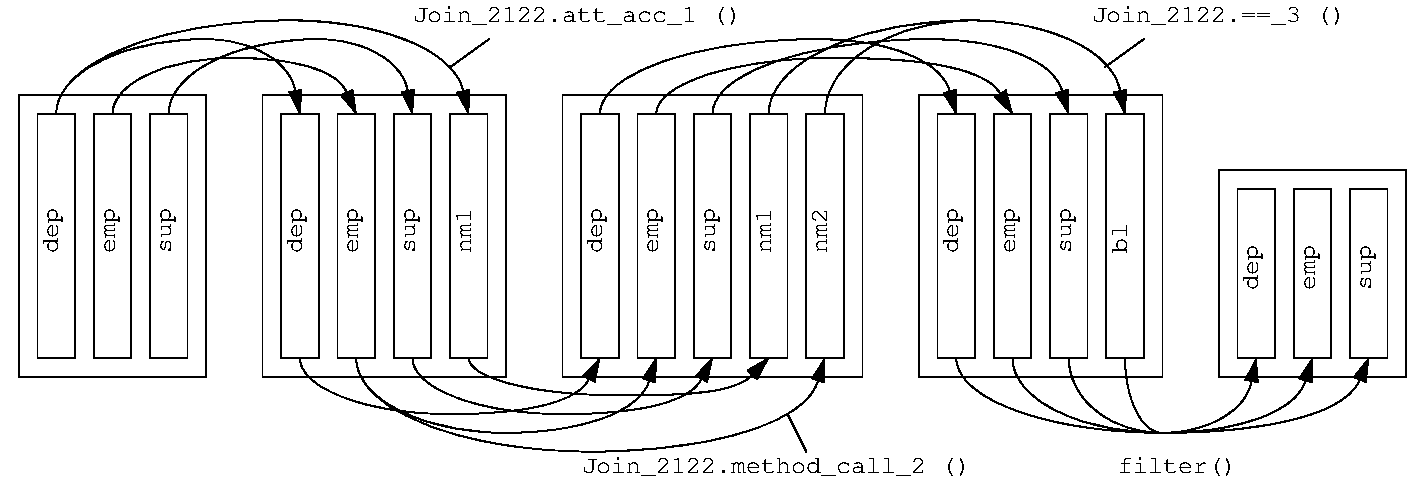
\includegraphics[width=3.3in]{TCAP}
  \end{center}
  \caption{Execution of the first four stages of a pipeline constructed from the example TCAP program.  The first two stages extract new vectors from 
existing vectors of objects, first via a call to
\texttt{Join\_2122.att\_acc\_1()}, which extracts
\texttt{Dep.deptName} from each item in the vector \texttt{dep}
of \texttt{Dep} objects, producing a new vector called \texttt{nm1}. Then,
via a call to \texttt{Join\_2122.method\_call\_2()}, which invokes \texttt{Dep :: getDeptName()} on each of the \texttt{Emp} objects
in the vector \texttt{emp}, producing a new vector called \texttt{nm2}.  A bit vector \texttt{bl} is formed by checking the equality of those two 
vectors via a call to \texttt{Join\_2122.==\_3()}, and then all of the vectors are filtered.}
  \label{fig:TCAP}
\end{figure}


\subsection{TCAP and Vectorized Execution} \label{sec:vectorized}

PC's vectorized execution engine repeatedly pushes 
so-called \emph{vector lists} through a series of pipeline stages.  Each pipeline stage
takes as input a vector list,
and produces a 
new vector list that consists of zero or more vectors from the input
vector list, as well as one or more vectors appended at the end of the list.
Pipeline stages are constructed in such a way that the overhead of a
virtual function call can be amortized on a vector list of objects,
aside from any virtual function calls that may be
present 
%(explicitly or perhaps implicitly in the form of memory management) 
in the user's code.
The TCAP language describes both the pipeline stages required to perform a PC computation, as well as the schema for each of the vector lists that
will be produced during the PC computation, and how each of the pipeline stages adds or removes vectors from the vector lists that are pushed through
the computation.

To see how this works through an example, consider a variant of the \texttt{getSelection()}:

\begin{codesmall} 
Lambda <bool> getSelection (Handle <Dep> arg1, 
     Handle <Emp> arg2, Handle <Sup> arg3) {
	return makeLambdaFromMember (arg1, deptName) == 
	       makeLambdaFromMethod (arg2, getDeptName); }
\end{codesmall}

\noindent PC compiles the lambda term resulting from a call to \texttt{getSelection()} into the following TCAP code:

\begin{codesmall}
WDNm_1(dep,emp,sup,nm1) <= APPLY(In(dep), 
   In(dep,emp,sup), 'Join_2212', 'att_acc_1', 
      [('type', 'attAccess'), ('attName', 'deptName')]);

WDNm_2(dep,emp,sup,nm1,nm2) <= APPLY(WDNm_1(emp), 
   WDNm_1(dep,emp,sup,nm1), 'Join_2212',
      'method_call_2', [('type', 'methodCall_2'), 
          ('methodName', 'getDeptName')]);

WBl_1(dep,emp,sup,bl) <= APPLY(WDNm_2(nm1,nm2),
   WDNm_2(dep,emp,sup), 'Join_2212', '==_3', 
      [('type', 'equalityCheck')]);

Flt_1(dep,emp,sup) <= FILTER(WBl_1(bl), 
   WBl_1(dep,emp,sup), 'Join_2212', []);
\end{codesmall}

\noindent
These four TCAP statements correspond to a pipeline of four stages,
as shown above in Figure \ref{fig:TCAP}.

This particular TCAP code begins with an \texttt{APPLY} operation, which is a five-tuple, consisting of: (1) the vector list and constituent
vector(s) for the \texttt{APPLY} to operate on, (2) the vector(s) from that vector list to copy
from the input to the output, (3) the name of the computation that the operation was compiled from, (4) the name of the compiled code (pipeline stage)
that the operation is to execute, plus (5) a key-value map that stores specific information about the operation that may be used 
later during optimization.

Specifically, in this case, the first \texttt{APPLY} in the TCAP computation describes a pipeline stage that
takes as input 
a vector list called \texttt{In}, which is made of the constituent vectors, referred to using 
the names \texttt{dep}, \texttt{emp}, and \texttt{sup}.
To produce the output vector list (called \texttt{WDNm\_1}), the vectors
\texttt{dep}, \texttt{emp}, and \texttt{sup} should be simply copied
(via a shallow copy similar with pointer assignment) from \texttt{In}.
In addition, the compiled code referred to by \texttt{Join\_2212.att\_acc\_1} will be executed via a vectorized application to the input
vector \texttt{dep}.  The result will then be put into a new vector called 
\texttt{WDNm\_1.nm1}.
The resulting vector list (consisting of the vectors shallow copied from the input as well as the new vector \texttt{WDNm\_1.nm1})
will be called \texttt{WDNm\_1}.  

Next, this TCAP program
specifies that \texttt{WDNm\_1} is processed by \texttt{APPLY}ing the
method call \texttt{getDeptName()} on the attribute \texttt{emp}; this is 
done via application of the compiled code referred to by \texttt{Join
  \_2212.method\_call\_2}.  
The vectors \texttt{dep}, \texttt{emp}, \texttt{sup}
and \texttt{nm1} are simply shallow-copied to the output vector list.

Then an equality check is performed to create \texttt{WBl\_1.bl}
(a vector of booleans) and the result is filtered based upon this
column.


Note that in each TCAP operation, the key-value map is only
informational and does not affect its execution.  However, this
information can be vital during optimization.  

\subsection{Template Metaprogramming}

In PC,
each vectorized pipeline stage (such as \texttt{Join\_2212.att\_ acc\_1}) is executed as fully-compiled native code, with no virtual function
calls.
In PC's C++ binding, this is accomplished by using the C++ language's extensive \emph{template metaprogramming} 
capabilities \cite{josuttis2012c++}.  Templates are the C++ language's way of providing generics functionality.
When a C++ template class or
function is instantiated with a type, %the instantiated template 
the C++ compiler actually generates optimized native code for that specific new type, at compile time.  
This is quite different from languages
such as Java, that must typically rely on slow virtual
function calls in order to implement generics.

To see how template metaprogramming is used by PC, consider
the TCAP operation from our example:

\begin{codesmall}
WBl_1(dep,emp,sup,bl) <= 
   APPLY(WDNm_2(nm1,nm2),WDNm_2(dep,emp,sup), 
      'Join_2212', '==_3', '');
\end{codesmall}

\noindent
Here, the pipeline stage \texttt{Join\_2212.==\_3} that is specified by the \texttt{APPLY} operation
actually refers to a function generated as a by-product of the
PC's \texttt{==} operation
in the line of code:

\begin{codesmall} 
return makeLambdaFromMember (arg1, deptName) == 
    makeLambdaFromMethod (arg2, getDeptName); 
\end{codesmall}

\noindent The \texttt{==} 
operation (corresponding to a higher-order function that
constructs a lambda term checking for equality in the output of two input lambda terms) is actually implemented as C++ template
whose two type parameters \texttt{LHSType} and \texttt{RHSType} are inferred from
the output types of the two input lambda terms. 
The \texttt{==} template returns an object of type \texttt{EqualsLambda} \texttt{<LHSType,} \texttt{RHSType>}, which
itself has an operation returning a pointer to the pipeline stage \texttt{Join\_2212.==\_3} referred to in the TCAP.
As expected, this stage processes in an input vector list,
creating a new vector of booleans, containing the truth values of the equality check of each \texttt{LHSType} from the left
input vector and each \texttt{RHSType} from the right input vector.
Using C++'s template metaprogramming facilities, this 
pipeline stage is generated specifically for \texttt{LHSType} and \texttt{RHSType} and optimized by the compiler for use with those
two types.  
As the \texttt{Join\_2212.==\_3} pipeline stage loops over the objects in the input vectors, 
there are no function calls that cannot themselves be inlined by the compiler
and optimized---unless, of course, the (potentially) user-defined equality operation over \texttt{LHSType} and \texttt{RHSType}
objects itself contains a virtual function call.

\eat{
\subsection{$k$-Means Example}

Now that we have described PlinyCompute at a high level, we turn to an example of what PlinyCompute looks like to a programmer.

Imagine that a user wished to use PC to build a high-performance library implementation of a $k$-means algorithm.
Once the programmer had defined the basic type over which the clustering is to be performed (such as the
\texttt{DataPoint} class), 
a programmer would likely next define a simple class that allows the averaging of vectors:

\begin{codesmall}
class Avg : public Object {
	long cnt = 1;
	Handle <Vector <double>> data = nullptr;
	Avg &operator + (Avg &addMe)
           {/* add addMe into this */}
};
\end{codesmall}

\noindent
The programmer might next add a method to the \texttt{DataPoint} class that converts the \texttt{DataPoint} object to an \texttt{Avg} object:

\begin{codesmall}
Avg DataPoint :: fromMe () {
	Avg returnVal;
	returnVal.data = data;
	return returnVal;
}
\end{codesmall}

\noindent
And also add a method to the \texttt{DataPoint} class that accepts a set of centroids, computes the Euclidean distance to
each, and returns the closest:

\begin{codesmall}
long DataPoint :: getClose (Vector <Vector <double>> 
        &centroids) {...}
\end{codesmall}

\noindent
Next, a programmer using PC would define an \texttt{AggregateComp} class using PC's lambda calculus, since, after all, the $k$-means algorithm is essentially 
an aggregation:

\begin{codesmall}
class GetNewCentroids : public AggregateComp 
    <Centroid, long, Avg, DataPoint> {

public:
   Vector <Vector <double>> centroids;

   Lambda <long> getKeyProjection (
       Handle <DataPoint> aggMe) override {
          return makeLambda (aggMe, 
              [&] (Handle <DataPoint> &aggMe) 
                 {return aggMe->
                     getClose (centroids);});
   }
   Lambda <Avg> getValueProjection (
       Handle <DataPoint> aggMe) override {
          return makeLambdaFromMethod 
              (aggMe, fromMe);
   }
};
\end{codesmall}

\noindent 
The declaration \texttt{AggregateComp <Centroid, long, Avg, DataPoint>} means that this computation aggregates
\texttt{DataPoint} objects.  For each data point, it will extract a key of type \texttt{long}, a value of type \texttt{Avg}, which will be
aggregated into objects of type \texttt{Centroid}.  To process each data point, the aggregation will use the lambdas constructed by
\texttt{getKeyProjection} and \texttt{get ValueProjection}.  
In this case, for example,
\texttt{getKeyProjec tion} builds a lambda which simply invokes the native C++ lambda given in the code---this
native C++ lambda returns the identity of the centroid closest to the data point.

To build a computation using this aggregation class, a programmer would need to specify the \texttt{Centroid} class (the result of this aggregation):

\begin{codesmall}
class Centroid : public Object {
	long centroidId; 
	Avg data;
public:
	long &getKey () {return centroidId;}
	Avg &getVal () {return data;}
};
\end{codesmall}

\noindent
And then build up a computation using these pieces:

\begin{codesmall}
Handle <Computation> myReader = 
    makeObject <ObjectReader <DataPoint>>
     ("myDB", "mySet");
Handle <Computation> myAgg = makeObject 
    <GetNewCentroids> ();
myAgg->centroids = ... // initialize the model
myAgg->setInput (myReader);
Handle <Computation> myWriter =  makeObject <Writer
     <Centroid>> ("myDB", "myOutSet");
    myWriter->setInput (myAgg);
pcContext.executeComputations (myWriter);
\end{codesmall}

\noindent After execution, the set of updated centroids would be stored in \texttt{myDB.mySet}.
Performing this computation in a loop, where the centroids are repeatedly updated until convergence, completes the implementation.


In our experience, for many applications such as Linear Algebra
Library, TPCH queries, or KMeans, PC codes require similar work in
terms of lines of source code to develop compared with equivalent codes using Spark's Scala binding, for
example, but require much lower effort to develop than using
object-oriented, C++ code without a declarative interface.

}



\section{Preliminary Experimental Evaluation}

In this section, we describe some preliminary experimental results, with the aim of demonstrating
to the
reader of the potential utility of the approach taken in the design and implementation of PC.

\vspace{5 pt}
\noindent
\textbf{Construction of a linear algebra library.}  Since PC is designed to support the construction
of high-performance tools and libraries, our first benchmarking effort was aimed at determining 
whether PC is actually useful for that task.  Thus, we asked
a graduate student who knew nothing of PC to use the system to build a small Matlab-like 
programming language and library for distributed matrix operations.
We called this implementation \texttt{LilLinAlg}.
Our goal was to determine the 
performance and functionality that an expert programmer (but PC novice) could deliver in a short
timeframe, compared to a set of established distributed Big Data matrix implementations:
SciDB \cite{brown2010overview, stonebraker2011architecture} (built from the ground up by an MIT team over the last nine years), MLLib \cite{meng2016mllib} 
(the Big Data matrix
implementation shipped with Spark), and SystemML \cite{boehm2014hybrid, ghoting2011systemml, boehm2016systemml}
(a matrix and machine learning implementation developed
over the last seven years by a team at IBM, built on top of Spark and Hadoop).
The student spent about six weeks in this effort.

We ran three different computations:
a Gram matrix computation (given a matrix $\textbf{X}$, compute
$\textbf{X}^T \textbf{X}$), least squares linear regression (given a matrix of features $\textbf{X}$ and
responses $\textbf{y}$, compute 
$\hat{\pmb{\beta}} = (\textbf{X}^{T} \textbf{X})^{-1} \textbf{X}^{T} \textbf{y}$), and nearest
neighbor search in a Riemannian metric space \cite{lebanon2006metric} encoded by matrix $\textbf{A}$ (that is,
given a query vector
$\textbf{x}'$ and matrix $\textbf{X}$, find the $k$ rows in the matrix that minimize 
$d_{\textbf{A}}^2(\textbf{x}_i, \textbf{x}') = 
(\textbf{x}_i - \textbf{x}')^T\textbf{A}(\textbf{x}_i - \textbf{x}')$).  All experiments used
ten Amazon
EC2 m2.4xlarge machines.  For
all three computations, 
$10^6$ data points were used.  Results are given in 
Table \ref{fig:LR} (for Gram and regression, SystemML V0.9 on Hadoop was used; for
nearest neighbor, V1.0 on Spark was used).


\begin{table}[h!]
\begin{center}
\begin{tabular}{|c||c|c|c||c|c|c||c|c|c||}
\hline
& \multicolumn{3}{c||}{Gram Matrix} & \multicolumn{3}{c||}{Linear Regression} & \multicolumn{3}{c||}{Nearest Neighbor} \\
\hline
Dimensionality & $10$ & $10^2$ & $10^3$& $10$ & $10^2$ & $10^3$& $10$ & $10^2$ & $10^3$ \\
\hline
\hline
PC (\texttt{LilLinAlg}) &00:07 & 00:09 &00:39 &00:14 &00:22 &00:49& 00:15 & 00:20 & 01:06 \\
SystemML &00:05$*$ &00:51 &02:34 &00:06$*$ &00:53 &02:38 &00:04$*$ &00:30 &01:32 \\
Spark \texttt{mllib} &00:20  &00:54 &17:31 &00:35 &01:01 &17:42 &01:20 & 04:49 &14:30 \\
SciDB   &00:03 &00:17 &03:20 &00:15 &00:33 &06:04 &00:28 &02:56 & 06:24 \\
\hline
\end{tabular}
\caption{Linear algebra benchmark. Format is MM:SS.
A star ($*$) indicates running in local mode.}
\label{fig:LR}
\end{center}
\end{table}

\vspace{-20 pt}
In every case except for the small problems when SystemML chose not to distribute the data,
\texttt{LilLinAlg} was the fastest.  
Though SystemML nearest neighbor approached the speed of 
\texttt{LilLinAlg}, we point out the vast difference in engineering effort between the two systems.  
SystemML was built over many years by a team of PhDs. Research papers have been written about the
technology developed for the system, including one awarded a VLDB best paper award \cite{boehm2016systemml}.
\texttt{LilLinAlg} was developed in six weeks, and it is faster (though to be fair, SystemML has a much broader
set of capabilities than \texttt{LilLinAlg}).

\vspace{5 pt}
\noindent
\textbf{Big object-oriented data manipulation.}
For an example of the raw performance of the PC object model and its ability to power large-scale 
object-oriented computations, we use the TPC-H benchmark data set \cite{council2008tpc}
and de-normalize
the data into a large set of \texttt{Customer} objects. Each
\texttt{Customer} object contains, among
other data, a list
or \texttt{Order} objects, and each \texttt{Order} object contains a list of \texttt{Lineitem} objects,
each of which has a \texttt{Part} and \texttt{Supplier} object.  
We run two computations. First, we compute, for each supplier,
the set of parts that the supplier has sold to each customer (stored
as a map from customer name to a list of part identifiers).
Second, we compute the $k$ customers whose set of \texttt{Part} items purchased is closest to
a query set, according to Jaccard similarity.
Because the data are object-oriented, it
is not possible to use Spark's Dataset/DataFrame abstraction to implement this computation, and so
we compare algorithmically equivalent Spark RDD and PC implementations.
Results are in Table \ref{fig:TPC}, run on the same 10 machine cluster.  

\begin{table}[h!]
\begin{center}
\begin{tabular}{|c||c|c|c|c|c|c|}
\hline
Kryo data size: &41.5GB & 83.1GB & 167.2GB &251.1GB &333.2 &416.2GB \\
\hline
& \multicolumn{6}{c|}{\texttt{Customer}s per \texttt{Supplier}} \\
\hline
PlinyCompute: hot PDB & 00:11&	00:19&	00:35&	00:51&	01:08&	01:21 \\
Spark: hot HDFS & 01:04&	01:53&	03:24&	04:54&	06:25&	08:16\\
Spark: in-RAM RDD & 00:16& 	00:29& 	00:56& 	01:21& 	02:18& 	03:56\\
\hline
& \multicolumn{6}{c|}{top-$k$ Jaccard} \\
\hline
PlinyCompute: hot PDB & 00:03&	00:03&	00:04&	00:05&	00:05&	00:06 \\
Spark: hot HDFS & 00:56&	01:38&	03:01 & 04:01&	05:22&	06:34\\
Spark: in-RAM RDD & 00:08& 	00:12& 	00:21 & 00:32& 	01:11& 	02:38\\
\hline
\end{tabular}
\caption{PlinyCompute vs. Spark for large-scale OO computation. Times in MM:SS.}
\label{fig:TPC}
\end{center}
\end{table}

\vspace{-20 pt}
We see that in a somewhat fair comparison, when PC data are
stored in a hot Pliny Database (PDB for short; PDB is PC's backend storage system) and Spark data
are stored in
a hot HDFS, the computation is $6\times$ to $66\times$ faster in PC.  We say ``somewhat'' fair
because at the end of the computation, Spark is left with a large number of objects that still need to be 
garbage collected by the JVM---a cost not included in the computation. If the data are already
fully deserialized and stored as an RDD, PC is 
between 50\% and $26\times$ faster.  However, we point out that this is not an apples-to-apples comparison.
Among other costs, it ignores
the cost Spark would incur at a later time to free the objects stored in RAM.

\vspace{5 pt}
\noindent
\textbf{Machine learning.}
Finally, we describe our experience writing a word-based, non-collapsed LDA implementation \cite{jermaineExperimental} on top of
both Spark and PC.  LDA is a standard text mining algorithm and non-collapsed LDA is chosen because
it is challenging:
it contains two joins and two aggregations among other operations.
Our Spark combined RDD and DataSet        
implementation was carefully engineered by an expert.
On the cluster used before, we run LDA over a 2.5 million document database.  Results (per iteration) are:

\begin{table}[h!]
\begin{center}
\begin{tabular}{|c||c|c|c|c|c|c|}
\hline
PlinyCompute & \makecell{Spark 1: \\vanilla} & \makecell{Spark 2: also with \\join hint} & \makecell{Spark 3: also with \\forced persist} & \makecell{Spark 3: also hand-\\coded multinomial} \\
\hline
02:05 & 50:20 & 17:30 & 09:26 & 05:00 \\
\hline
\end{tabular}
\caption{PlinyCompute vs. Spark for LDA. Times in MM:SS, averaged over five iterations.}
\label{fig:LDA}
\end{center}
\end{table}

\vspace{-20 pt}
While Spark performed well---in the end, PC was somewhat
limited by the lack of engineering that has gone
into its broadcast protocol---the 
amount of work required to arrive at a good solution 
was significant, representing about a week of tuning.  First, among other things, our Spark expert had to force a 
broadcast join.  Then, it was necessary to force Spark to
persist the result of one of the joins for later use.  Finally, it was necessary to hand-code a 
Multinomial sampler to obtain an implementation that was competitive with PC.
This illustrates the advantage of PC's declarative approach: decisions such as broadcast vs. full hash
join as well as which intermediate results to materialize are automated.  




\section{Proposed Research Plan}

We now turn to the set of research
problems that will be addressed by the proposed project.

\subsection{Optimization of Very Large Computational Plans}

\noindent
\textbf{Problem description.}
A typical PC application builds up a graph of \texttt{Computation} objects (\texttt{JoinComp}, \texttt{SelectionComp}, etc.).  
This graph can be very large, especially for machine learning.  For example, 
processing a layer in a forward pass in a deep feedforward network can take five operations, with seven
in the backward pass.  Ten backpropagation iterations over a ten-layer network is more than one thousand operations.

PC relies on automatic, relational database-style optimization to choose the correct plan for such a computation.
Unfortunately, it is difficult to optimize very large graphs---performing logical optimizations such as 
changing join orders, as well as physical optimizations such as pipelining operations into one another and choosing implementation
algorithms.  Classical cost-based
relational techniques \cite{selinger1979access} break down after more than a few dozen operations \cite{graefe1993volcano}.
An obvious solution is to cut the graph into manageable pieces, and optimize and execute each piece separately.
The problem is that such a cut can be arbitrarily bad.  For example, in \texttt{LilLinAlg},
a multiplication of matrices \texttt{A} ($n\times m$ sub-blocks)
and \texttt{B} ($m\times p$ sub-blocks) 
produces $n \times m \times p$ blocks from a join, which is followed by an aggregation.  If pipelined into the aggregation, that set
of blocks is never materialized---it is streamed across the network and immediately aggregated.  
But if we are unlucky enough to cut the graph so as to separate the aggregation and the
join, we will materialize a huge intermediate result.  This is debilitating.

\vspace{5 pt} 
\noindent
\textbf{Proposed approach.}
We plan to formalize the problem of breaking a large computational plan into a set of \emph{frames}, or connected sub-plans.
Each frame is optimized and executed separately, and its output materialized.
It is possible
to write the problem of producing a ``good'' partitioning
as an integer program, where the goal is to produce a set of frames such that no frame exceeds an input maximum size.
This is done so as to minimize the value of a cost function that measures the cost incurred by the cut.
Different
costs are incurred by separating different types of operations.  Separating an aggregation from a subsequent operation
is generally low cost---aggregation tends to reduce output size, and it is blocking and cannot be pipelined. So forcing
such a result to be materialized is not often problematic.
But separating
a selection from either the operation before it or after it is high cost; it is always possible to pipeline though a selection, and
so cutting before or after a selection necessarily requires an un-necessary materialization.  

\vspace{5 pt}
\noindent
\textbf{Research Questions.}  There are several obvious research questions.  First, this particular IP formulation is NP hard.  Can
we develop heuristics to solve it effectively?  Also, how to choose the various weights?  They can be chosen through trial and error
or thought experiment and shipped with the system, but are there better methods?  Might we develop methods that can learn
over time?
What information should be passed across frames?  How do we recognize when an operation in one frame must have the same output
size as an operation in another frame?  In many ways, this resembles the query containment problem \cite{calvanese1998decidability, kolaitis1998conjunctive}.
Can we leverage the fact that, especially in machine learning computations, various patterns are repeated
iteratively?
That is, can we develop a method that uses already-observed information to improve the solution?

\subsection{Statistical Models for Combined Execution and Optimization}

\noindent
\textbf{Problem description.}
Classical, cost-based methods for optimizing computations do not necessary apply over opaque user code.
While PC may understand that
a particular operation such as a \texttt{JoinComp} is checking for equality across two sets (due to the programmer's
use of the \texttt{==} operation
in PC's Lambda calculus) and it will even understand where the values are coming from (an opaque C++ lambda, a method call, an attribute,
etc.), PC will \emph{not} have the key statistics, such as the number of unique values returned from an opaque C++ lambda, 
that are typically used for estimating the size of a join.  

\vspace{5 pt} 
\noindent
\textbf{Proposed approach.}
Optimizing in the face of this sort of uncertainty presents a classical exploration/exploitation tradeoff \cite{kocsis2006bandit}. 
One can  
execute a computation (or partially execute a computation) in order to obtain a set of statistics, and then optimize the 
remainder of the compute plan after obtaining the
statistics, or one can simply jump into the computation, and do the best job possible with the information at hand.  The former is
exploration, and the latter is exploitation.  Exploration has a cost, as stopping to plan means that opportunities for optimization,
such as pipelining, are lost.  We model the task of optimizing in the face of uncertainty as a 
Markov Decision Process (MDP) \cite{cassandra1998exact, white1991survey}.  Each state in the MDP consists of the portion of a computation that has been executed, the portion
left un-run, and the set of statistics that have been collected.  If one includes information such as a prior distribution over
the various statistics such as the number of distinct values, it is possible to compute the expected reward of moving to a new state 
by integrating over the value of each statistic.  However, this is computationally very difficult---even using Monte Carlo methods for
the integration \cite{littman1995complexity}---as it also requires optimizing the plan in the face of every possible value for the statistic.

As an alternative to solving the MDP precisely, we instead plan to apply deep reinforcement learning (deep RL) \cite{mnih2015human, lillicrap2015continuous, mnih2013playing} to the problem.  
Specifically, we will give the RL algorithm access to an encoding of the computational plan as well as the various statistics that
have been collected, the various choices for the next operation to run, as well as estimates for the cost of each of the operations,
as functions of the statistics.  By actually allowing the algorithm to make choices and execute parts of the computation and
then obtain feedback in the form of running time that is backpropagated through the network, the hope is that it is possible to
learn how to co-manage the collection of statistics and execution.

One of the fundamental problems with this approach is that RL can take a very long time to learn an effective policy, especially
in a rich environment.  It is likely impractical to actually learn
by running computations on top of PC, which can take a long time. 
Thus, our plan is to train
via 
simulation.  That is, we will build a simulator and synthesizer for synthetic computations that draws statistics from user-specified
priors, and use that to train the deep RL algorithm.

\vspace{5 pt}
\noindent
\textbf{Research questions.}  
Deep RL is often difficult to use in practice.
What exactly is th deep RL formulation?  How is the problem space to be encoded?  What do the deep networks look like?
Many formulas regarding the complexity of running
relational operations are known; how should those be incorporated into the RL?  
How does one synthesize reasonable computations for training the RL?

\subsection{Developing Support for Cross-Block References}

\noindent
\textbf{Problem description.}
One of the most important ideas in the design and implantation of PC is that all allocations are \emph{in place}, obviating the
need to ever serialize or deserialize PC \texttt{Object}s.  In order to support this, all PC \texttt{Handle}s by definition
point within a page, so \texttt{Handle} dereferences are always valid, even after a page moves across processes.
One difficulty is that cross block assignments often happen.  For example, we may have:
\texttt{Handle <Vector <Handle <DataPoint>}\texttt{>}\texttt{>} 
\texttt{myVec} \texttt{=} \texttt{makeObject <Vector <Handle <DataPoint>>> ();}.
By definition, \texttt{myVec} is now
stored in the thread's current allocation block.  Imagine that \texttt{storeMe} was
declared as \texttt{Handle <DataPoint>} and pointed to a PC \texttt{Object} that had just been read over the network.  The line of code
\texttt{myVec->push\_back (storeMe);}
will automatically deep copy the PC \texttt{Object} pointed 
to by \texttt{storeMe} to the current allocation block, preserving zero cost data movement.
When a deep copy fails due to lack of space, a fault occurs, the copy is undone, and the application (or, more likely, PC itself)
deals with the over-full page in an appropriate manner.

The problem with this is that sometimes, it is desirable to \emph{allow} cross-block \texttt{Handle}s.  
Always performing deep copies and forcing only within-block \texttt{Handle}s incurs a cost due to the copy.  It also seriously
limits the
size of an \texttt{Object} graph that a programmer can create, since graphs that are larger than a single page cannot be moved
across machines or to storage.  
Graph-based Big Data programming models have become popular, where programmers access data by traversing links, and we wish to 
support this.

\vspace{5 pt} 
\noindent
\textbf{Proposed approach.}
If one allows out-of-block \texttt{Handle}s, the key problem becomes dealing with faults efficiently.  
How does one ensure that when an out-of-page PC \texttt{Handle} is dereferenced,
the data it points to is accessed efficiently, perhaps across the network, without wasted CPU cycles? 
The key idea we wish to explore is \emph{latency masking}, closely related to the methods used in classical context switching \cite{silberschatz2014operating}.  
Because all PC computations logically operate in parallel over the items in a large set,
it may be possible to react to a fault 
by saving the state 
of the computation for the current PC \texttt{Object}, requesting the data transfer,
and moving onto the next \texttt{Object}. There is typically always another \texttt{Object} to process, 
and by definition, PC \texttt{Object}s can 
be processed in any order.  Each computation that causes
each fault is saved, and then resumed when the referenced \texttt{Object}'s page is retrieved.
Note that the key difference between this approach and classical applications of context switching that the contexts being saved
are within the same process and, in fact, the same thread---each context
is associated with the processing of a particular PC \texttt{Object}.

\vspace{5 pt} 
\noindent
\textbf{Research questions.} 
One key question is: is it possible to avoid such faults entirely by pre-fetching the targets of \texttt{Handle}s before they are
ever accessed?  Specifically, when a PC \texttt{Object} with a \texttt{Handle} is loaded into RAM, is it possible to develop a policy that
can be used to pre-fetch the \texttt{Object} in the background, before a fault occurs?
Also, since all PC computations are functional, they can be run and re-run without side effects (except for possible memory leaks
if the programmer uses C-style allocations).  This means that another option is simply killing the computation being run over an
\texttt{Object} when a fault occurs, loading the requested page, and then re-starting the computation, which will then run without fault.
This has the benefit that no state need be saved.
When to save context, and when to re-run?  

\subsection{Continuous Computations}

\begin{figure}[t]
  \begin{center}
    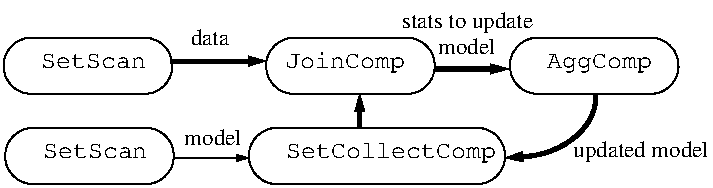
\includegraphics[width=4in]{ParamServer}
  \end{center}
\vspace{-10 pt}
  \caption{A parameter server using PlinyCompute.  Bolded links are those labeled as \texttt{continuous}.}
  \label{fig-param}
\vspace{-15 pt}
\end{figure}


\noindent
\textbf{Problem description.}
One of the most important applications for any distributed compute platform is machine learning, and
there is sometimes a significant
benefit to asynchronous computation in ML \cite{mnih2016asynchronous, dean2012large}.
Asynchronous computation may
result in models with lower error, as asynchronous training is less likely to over-fit the training data.  
Much work in asynchronous distributed machine learning utilizes
a distributed \emph{parameter server} architecture \cite{li2014scaling, ho2013more}, 
where a set of workers each request a subset of the current
model from a ``parameter server'' (essentially, a key-value store).  The workers then use that model 
to perform a computation over a subset of the data set; this computation updates the model and sends
the updated model back to the parameter server.  This update is asynchronous in that
workers may all be operating on different versions of the model, and updating the model without coordination.

The problem is that the programmer burden for writing a parameter server code is very high for anything other than
simple data-parallel computation where each worker operates on a separate copy of the model.  
Further, automatically-generated learning algorithms (such as those created by TensorFlow's automatic differentiation capabilities)
are unable to generate anything other than simple, data-parallel code when
often, complicated, model parallel implementations \emph{are} necessary.
Consider a large, deep neural network having 
two adjacent, fully connected layers of one million neurons.  This model requires a one-trillion entry
weight matrix.  Pushing
a batch of 100 data points through such a connection in one second
during training will require $2 \time 10^{14}$ FLOPS---the power in 20 high-end
GPUs---and the set of weights for an all-to-all connection will require more than a terabyte to store.
Such models must by definition be handled in parallel, but
developing such a code for a parameter server
is difficult at best.

Fortunately, orchestrating complex distributed computations of this sort on PC is quite easy.  Learning the weights
in the sort of application described above requires what amounts to distributed linear algebra, which is easy to implement on top of PC.

\vspace{5 pt} 
\noindent
\textbf{Proposed approach.}
That said, PC is purely a synchronous system.  To add asynchrony,
we will allow a programmer to label an output from one or more computations to be  
\texttt{continuous}.  Just like their non-continuous
versions, each
continuous computation represents a computation that produces a set of PC \texttt{Object}s.
However, the key difference is that a \texttt{continuous}-labeled 
computation is free to send any output \texttt{Object} computed from its current inputs
at any time.
This means that a \texttt{continuous}-labeled computation is forever updating and re-sending output \texttt{Object}s.

Each computation producing a \texttt{continuous}-labeled output must declare a key for the output \texttt{Object}s.  When
two output \texttt{Object}s with the same key are processed by any computation, the newer PC \texttt{Object} is removed, and the computation consuming
that set is responsible for updating its own output set with the new \texttt{Object}.  This update is asynchronous in the sense that
all computations are constantly updating their output sets in response to changes in their input, with no synchronization.

It is easy to simulate an asynchronous 
parameter server using these abstractions, as depicted in Figure \ref{fig-param}.  In this computational plan, data are
scanned continuously.  At the same time, the model is scanned into a \texttt{SetCollectionComp} and then joined with the 
data.  The computation that occurs in the \texttt{JoinComp}
corresponds to the computation done in a worker in a parameter server.
In the join, a set of statistics needed to update the model
are computed and aggregated---the result of the aggregation is the updated model.
As the updated model enters into the \texttt{SetCollectionComp}, it asynchronously replaces the initial model.  The current
state of the model is constantly re-sent into the join.  The cycle
repeats until convergence.

The benefit of this computation-centric view is that it is possible to build
complex computations with little effort.  A model-parallel computation---where a very large model is distributed across the cluster
is easily implemented.  For example,
a forward-backward pass through a deep network utilizing a series of distributed matrix multiplies corresponds
to a series of \texttt{JoinComp}--\texttt{} pairs.

Note that this looks a lot like continuous or stream-based query processing in database systems.  The key difference is that rather
than processing queries over sliding windows (as is typical in stream-based processing), query processing is done over constantly
updated sets.

\vspace{5 pt}
\noindent
\textbf{Research Questions.}  Building such functionality into PC will be challenging.
One key research challenge is how to efficiently perform online updates to query result sets---this looks
something like the materialized view maintenance problem from database systems \cite{gupta1995maintenance, agrawal1997efficient}.  We will investigate how to attach lineage 
to cached results \cite{buneman2007provenance, widom2004trio}, in order to efficiently perform the required updates, and
leverage ideas from streaming systems \cite{zaharia2013discretized, babcock2002models}  and continuous query processing \cite{chandrasekaran2003telegraphcq, chen2000niagaracq}.
Another challenge is how to develop reasonable algorithms
for scheduling and
resource management---especially memory management---which
will be difficult since all operations in a plan are potentially active at the same time.  

\subsection{Developing PC-Specific Compiler Optimizations}

\noindent
\textbf{Problem description.}
As a final research problem, we will attempt to develop a set of compiler optimizations 
(over the LLVM IR \cite{lattner2004llvm}) that are
specific to PC.  Through experience, we have found that there 
are a number of performance errors that PC programmers make that could be fixed by a compiler, if the compiler were
aware of the semantics of PC computations.  For example,
in PC, dynamic method call dispatch over PC \texttt{Object}s (and in, fact, all automatic movement and dynamic loading 
of code in PC)
is facilitated by the type code stored within each
\texttt{Handle} object.
The
type code is a unique identifier for the PC-\texttt{Object}-descended type of the object that the \texttt{Handle} points to.

In every major C++ compiler (GCC, \texttt{clang}, Intel, and Microsoft), virtual functions
are implemented using a virtual function table, or \texttt{vtable} object, a pointer to which is located at the beginning
of each C++ object having a virtual function.  Unfortunately, the \texttt{vtable} pointer is a native, C-style pointer, and so the
\texttt{vTable} pointer does not automatically translate when an
object is moved from process to process.  To handle this, in
PC's C++ binding, whenever a PC \texttt{Handle} object is dereferenced,
a lookup on the
type code is performed transparently to the application programmer, and the \texttt{vTable} pointer in the PC \texttt{Object} is ``fixed''.
First, if necessary, a shared library containing 
the correct \texttt{vTable} is fetched from PC's catalog server and loaded into RAM, and then the  \texttt{vTable} pointer
in the PC \texttt{Object} is changed to point to the correct \texttt{vTable}.

The problem is that since the code associated with a \texttt{Handle} deference cannot be sure of its context---whether it must
have already been dereferenced---this lookup must happen at \emph{every} dereference.  Programmers often put such dereferences
with a loop, as they assume the dereference is costly. We find that sometimes, these lookups
can take up 30\% of the CPU cycles in a PC computation.

\vspace{5 pt} 
\noindent
\textbf{Proposed approach.}
A careful programmer can re-factor code to avoid multiple dereferences, performing the dereference once before entering the loop,
leading to a dramatic increase in performance.  However, even though the target programmer for PC is a capable systems developer,
this
is asking a lot of a programmer.  It would be much better for the compiler itself to recognize such situations, and to take
appropriate action.  There are many other, similar optimizations that could catch and remedy standard PC programming errors.
Our plan is to implement these optimizations as an LLVM plug-in.

\vspace{5 pt}
\noindent
\textbf{Research questions.} Our experience tells us that there are many such examples of optimizations that could help fix many
of the problems that users have when attempting to use the PC \texttt{Object} model effectively.
What is the set of PC-specific compiler optimizations that can remedy common performance problems?
Might we change the semantics of PC computations to allow more opportunities for optimization?

\subsection{Evaluation}

All of the ideas explored as part of the proposed research project will be implemented and evaluated as part of PC; any
ideas that prove to have merit will be released as part of PC. To
measure our progress,
we will also develop a set of benchmark codes on top of PC, in three categories: machine learning,
data processing, and linear algebra (a preliminary version of this benchmark was described in the Preliminary Experimental Evaluation
section of the proposal).  In machine learning, we have already begun porting TensorFlow \cite{abadi2016tensorflow} onto PC, using PC's execution engine
rather than TensorFlow's own parameter server; we will maintain a number of deep learning benchmarks comparing PC to the current
release of TensorFlow; we will also maintain current
results comparing LDA, Gaussian mixture modeling, K-means, and several other standard
machine learning algorithms to implementations on top of Spark and Flink.  In data processing, we will continue to develop
various queries on the denormalized TPC-H data set, and compare with Spark and Flink implementations.  And finally, we will
continue to develop \texttt{LinLinAlg}, and maintain results comparing its speed with \texttt{MLLib}, SystemML, and SciDB.





\section{Conclusions}

This paper has described PlinyCompute, or PC for short.  PC is a system for the development of high performance
distributed data processing tools and libraries.  PC is designed to inhabit the space between
high-performance computing platforms such as OpenMP and MPI, which provide little direct support
for managing very large data sets, and dataflow platforms such as Spark and Flink, which rely on 
a managed runtime to provide low-level services such as allocation and deallocation of data objects and memory management.
PC's guiding design principle is ``declarative in the large,
high performance in the small''.
In the large, PC presents the capable systems programmer with a very high-level, declarative interface, relying on automatic,
relational-database style optimization.  This is crucial for tool and library development, since the same tool should run well
regardless of the characteristics of the data and of the compute platform.  But in the small, PC relies on the PC object model.
The PC object model is an
API for storing and manipulating persistent data, and has been co-designed with PC's memory management
system and computational engine to provide maximum performance.
One of the key ideas behind the PC object model is the \emph{page as a heap principle}. All PC
Objects are allocated and manipulated in-place, on a system- (or user-) allocated page. There is no distinction
between the in-memory representation of data and the on-disk (or in-network) representation of data.
Thus there is no (de-)serialization cost to move data to/from disk and network, and memory management
costs are very low.

We have performed a reasonably extensive set of benchmark experiments that indicate that these ideas can result in 
a system that is very high performance and yet offers a relatively simple and usable object oriented API.  In particular, 
we have given strong evidence that PC \emph{is} particularly well-suited to tool and library development. 
For example, we asked a PhD
student (who at the outset knew nothing of PC) to use the system to build a small Matlab-like programming
language and library for distributed matrix operations called
\texttt{lilLinAlg}.  The resulting tool outperformed many other, long-lived tools
for the same purpose, such as SciDB, \texttt{mllib}, and SystemML.  SystemML in particular has resulted 
in several research papers,
including one awarded a VLDB best paper award \cite{boehm2016systemml}.
\texttt{lilLinAlg} was developed in six weeks by a single PhD student.
One may conjecture that had SystemML been built on a platform such as PC rather than on Spark, it might be significantly
faster than it is now.

Many avenues for future work remain.  In particular, there is significant scope for expanding the functionality and
usability of the PC object model, including relaxing the strict requirement that all \texttt{Handle}s point within a page.  This
would allow pointer-like objects to point off a page, perhaps even off of a machine.  


\newpage
\setcounter{page}{1}
\bibliographystyle{abbrv}
\bibliography{buds}

%\input{gmm}
%\input{analysis-detailed}

\end{document}
